\section{Multiresolution Analysis (MRA) oder Multiskalen-Analyse (MSA)}
\baeni{63}
MRA ist eine Designmethode für die diskrete Wavelet Transformation (DWT). Sie ist mit einem Mikroskop vergleichbar, durch welches man eine Funktion mit frei wählbarer Auflösung (Vergrösserung) an frei wählbarer Stelle betrachten kann.

\subsection{Orthogonal MRA}
Die Skalierungsfunktion (Father function $\varphi(t)$) ist vorstellbar als kurzen, mehrheitlich positiven Impuls und nicht zu verwechseln mit Wavelets (Mother function $\psi(t)$): 
\[
	\varphi_{m,n}(t)=2^{-m/2} \cdot \varphi(2^{-m}\cdot t - n) = \frac{1}{\sqrt{2^{m}}} \cdot \varphi(2^{-m}\cdot t -n) = 2^{-m/2} \cdot \varphi(2^{-m}\cdot (t - 2^{m}\cdot n))
\]

\textbf{Axioms} (Anforderungen) die eine Skalierungsfunktion erfüllen muss:
\begin{enumerate}
	\item Orthonormality: $ \langle \varphi_{0,n}|\varphi_{0,n'} \rangle = \delta_{n,n'} =  \begin{cases} 1 \quad n=n'\\ 0 \quad sonst  \end{cases}  $
	\item 2-scaling relation: $ \varphi(t) = \sqrt{2} \sum_{k \in \mathbb{Z}} h_k \cdot \varphi(2t-k) = \sum_{k \in \mathbb{Z}} h_k \cdot \varphi_{-1,k}(t) \qquad \varphi_{m,n}=\sum_{k \in \mathbb{Z}} h_k \cdot \varphi_{m-1,2n+k} $
	\item Mean one: $ \varphi \text{ muss integrierbar sein und } \int_{-\infty}^{\infty}\varphi(t) \mathrm{d}t = 1 $ (Wavelets $\psi(t)$ haben Mittelwert 0)
\end{enumerate}

(Aussage von 2-scaling relation: Eine Funktion wird um den Faktor 2 (in der Zeit) gestaucht. Durch verschieben, strecken bzw. stauchen (der Amplitude) und aufaddieren dieser skalierten Funktion, kann die  Ausgangsfunktion wieder dargestellt werden.)

Daraus ergeben sich folgende einfachen Konsequenzen:
\[ 
	\sum_{k \in \mathbb{Z}} h_k = \sqrt{2} \qquad \qquad (\text{z.B.: } h_0 + h_1 + h_3 + h_4 + h_5 = \sqrt{2})
\]
Double-Shift-Orthogonality:
\[
	\delta_{0,n} = \sum_{k \in \mathbb{Z}} h_k h_{k-2n} 
	\qquad \qquad 
	(\text{z.B.: } h_0h_2 + h_1h_3 + h_2h_4 + h3_h5 = h_0h_4+h_1h_5 = 0 )
\]

Scale space: 
\[
	V_m = \langle \varphi_{m,n}|n \in \mathbb{Z}  \rangle = \{ ...,\varphi_{m,-1},\varphi_{m,0}, \varphi_{m,1}, \varphi_{m,2},... \}
	\qquad \qquad
	V_mf = \sum_{n \in \mathbb{Z}} u_{m,n}\varphi_{m,n} \quad \text{mit } u_{m,n}=\langle \varphi_{m,n}|f \rangle
\]

Lokalisation:
\[  
	m \rightarrow -\infty \quad ||f-V_mf||^2 \rightarrow 0 \quad (\text{finer (feiner)})
	\qquad \qquad
	m \rightarrow +\infty \quad ||V_mf||^2 \rightarrow 0 \quad (\text{coarser (gröber)})
\]

Detail space (Detailinformation):
\[
	W_m = \langle \psi_{m,n} | n \in \mathbb{Z} \rangle = \{ ...,\psi_{m,-1},\psi_{m,0}, \psi_{m,1}, \psi_{m,2},... \}
	\qquad \qquad
	W_mf = \sum_{n \in \mathbb{Z}} \nu_{m,n}\psi_{m,n} \quad \text{mit } \nu_{m,n}=\langle \psi_{m,n}|f \rangle
\]
Räume (je weiter nach rechts (je kleiner m), desto grösser der Raum):
\[ V_{m-1} = V_m \oplus W_m  \qquad \qquad ...\subset V_{m+1} \subset V_{m} \subset V_{m-1} \subset ... \]

\textbf{Wavelet aus Skalierungsfunktion} \baeni{69}:
\[
	\psi_{m,n} = \sum_{k \in \mathbb{Z}} g_k \varphi_{m-1,2n+k} 
	\qquad \qquad 
	\left(\psi_{0,0}=\sum_{k \in \mathbb{Z}} (-1)^k h_{l-k} \sqrt{2}  \varphi_{0,0}(2t-k) = \sum_{k \in \mathbb{Z}} g_k \varphi_{-1,k} \quad \underbrace{l \in \mathbb{Z}_{ungerade}}_{\text{frei wählbar}} \right)
\]

\textbf{Fast Wavelet Transform} (Decomposition / Reconstruction, \baeni{73}):
\[
	\boxed{\begin{array}{ccccc}
		u_m & \xrightarrow{(\downarrow 2)A} & u_{m+1} & \xrightarrow{(\downarrow 2)A} & u_{m+2} \\
		& \searrow^{(\downarrow 2)D} & & \searrow^{(\downarrow 2)D} & \\
		& & \nu_{m+1} & & \nu_{m+2} \\
	\end{array}}
	\qquad \qquad \qquad \qquad
	\boxed{\begin{array}{ccccc}
		u_{m+2} & \xrightarrow{\tilde{A}(\uparrow 2)} \oplus& u_{m+1} & \xrightarrow{\tilde{A}(\uparrow 2)} \oplus & u_{m} \\
		& \nearrow_{\tilde{D} (\uparrow 2)} & & \nearrow_{\tilde{D} (\uparrow 2)} & \\
		\nu_{m+2}& & \nu_{m+1} & & \\
	\end{array}}
\]

\[  
	u_{m+1,n} = \sum_{k \in  \mathbb{Z}} h_{k-2n} u_{m,k} \quad \nu_{m+1,n} = \sum_{k \in  \mathbb{Z}} g_{k-2n} u_{m,k}
	\qquad \qquad
	u_{m,n} = \sum_{k \in  \mathbb{Z}} h_{n-2k} u_{m+1,k} + g_{n-2k} \nu_{m+1,k}
\]

\[
	A(x)_n = \sum_{k \in  \mathbb{Z}} h_{k-2n} x_k
	\qquad \qquad \qquad \qquad
	\tilde{A}(x)_n = \sum_{k \in  \mathbb{Z}} h_{n-2k} x_k
\]

\[
	D(x)_n = \sum_{k \in  \mathbb{Z}} g_{k-2n} x_k
	\qquad \qquad \qquad \qquad
	\tilde{D}(x)_n = \sum_{k \in  \mathbb{Z}} g_{n-2k} x_k
\]

\begin{tabular}{l r c l}
Upsampling
  & $(..., x_{-1}, \underline{x_0}, x_1, x_2, x_3, x_4, ...)$
  & $\xrightarrow{\uparrow 2}$
  & $(..., x_{-1}, 0, \underline{x_0}, 0, x_1, 0, x_2, 0, x_3, 0, x_4, 0, ...)$ \\
Downsampling
  &$(..., x_{-2}, x_{-1}, \underline{x_0}, x_1, x_2, x_3, x_4, ...)$ 
  & $\xrightarrow{\downarrow 2}$ 
  & $(..., x_{-2}, \underline{x_0}, x_2, x_4, ...)$
\end{tabular}


Vereinfachung des Analyseschritts für die Handrechnung $k-2n=l\rightarrow k=l+2n$:
\[ 
	u_{m+1,n} = \sum_{l} h_{l} u_{m,l+2n}
	\qquad \qquad \qquad \qquad
	\nu_{m+1,n} = \sum_{l} g_{l} u_{m,l+2n}
\]

\textbf{Beispiel Rekonstruktion} (Übung 6-2b):\\
Geg.:
$\underline{u} = \frac{1}{\sqrt{2}} ( \underline{3}, 7, 10, 13); \; 
\underline{\nu} = (\underline{\sqrt{2-3}}, 3\sqrt{2}-7, 5\sqrt{2}-10, 6\sqrt{2}-13);\;
\tilde{A} = (\underline{1}, \sqrt{2}-1)$\\
$\underline{\tilde{x}} = \tilde{A} * \left((\uparrow 2)(\underline{u}) \right) \oplus \tilde{D } * \left( (\uparrow 2) (\underline{\nu})\right)$\\
$\tilde{A} * \left((\uparrow 2) (\underline{u}) \right)= 
(\underline{1}, \sqrt{2}-1) * \frac{1}{\sqrt{2}}(\underline{3}, 0, 7, 0, 10, 0, 13) =
(\underline{\frac{3}{\sqrt{2}}}, 3-\frac{3}{\sqrt{2}}, \frac{7}{\sqrt{2}}, 7-\frac{7}{\sqrt{2}}, \frac{10}{\sqrt{2}}, 10-\frac{10}{\sqrt{2}}, \frac{13}{\sqrt{2}}, 13-\frac{13}{\sqrt{2}})$ \\
Analog zum \em Moving Average \em ($\tilde{A}$) erfolgt Berechnung der  \em Moving Difference \em ($\tilde{D}$). Schlussendlich Elementweise addieren.


\subsection{Biorthogonal MRA \baeni{76}}

\textbf{Axioms} (Anforderungen) die eine Skalierungsfunktion erfüllen muss:
\begin{enumerate}
	\item Biorthogonality: $ \langle \varphi_{m,n}|\tilde{\varphi}_{p,q} \rangle = \delta_{m,p}\cdot \delta_{n,q} \qquad \qquad \left( \langle \varphi_{0,n}|\tilde{\varphi}_{0,0} \rangle = \delta_{0,n} \right)$
	\item 2-Scaling relation: $ \varphi_{0,0}(t) = \sum_{k \in \mathbb{Z}} h_k \cdot \varphi_{-1,k}(t) \qquad \qquad  \tilde{\varphi}_{0,0}(t) = \sum_{k \in \mathbb{Z}} h_k \cdot \tilde{\varphi}_{-1,k}(t) $
	\item Mean one: $ \int_{-\infty}^{\infty}\varphi(t) \mathrm{d}t = 1 \qquad \qquad \int_{-\infty}^{\infty}\tilde{\varphi}(t) \mathrm{d}t = 1$
\end{enumerate}

Einfache Konsequenzen sind:
\[ 
	\sum_{k \in  \mathbb{Z}} h_k = \sum_{k \in  \mathbb{Z}} \tilde{h}_k = \sqrt{2} 
	\qquad \qquad
	\text{Double shift orthogonality:} \quad \sum_{k \in  \mathbb{Z}} h_k \tilde{h}_{k+2n} = \delta_{0,n}
\]

$  
	\text{Analyse-Funktion: } \varphi_{m,n} \quad \psi_{m,n}
	\qquad \qquad
	\text{Synthese-Funktion: } \tilde{\varphi}_{m,n} \quad \tilde{\psi}_{m,n}
$

\vspace{2mm}

\textbf{Wavelet aus Skalierungsfunktion}:
\[
	\psi_{0,0}=\sum_{k \in \mathbb{Z}} (-1)^k \tilde{h}_{l-k} \sqrt{2}  \varphi_{0,0}(2t-k) = \sum_{k \in \mathbb{Z}} g_k \varphi_{-1,k} 
	\qquad
	\tilde{\psi}_{0,0}=\sum_{k \in \mathbb{Z}} (-1)^k h_{l-k} \sqrt{2}  \tilde{\psi}_{0,0}(2t-k) = \sum_{k \in \mathbb{Z}} \tilde{g}_k \tilde{\psi}_{-1,k} 
	\qquad 
	\underbrace{l \in \mathbb{Z}_{odd}}_{\text{frei wählbar}}
\]


\subsection{Filterbank Beschreibung \baeni{45}}
Up-/ Downsampling: $ S(z) (\downarrow 2)(\uparrow 2) = \frac{1}{2} (S(z)+S(-z) $

\vspace{-2cm}

\begin{flushright}
	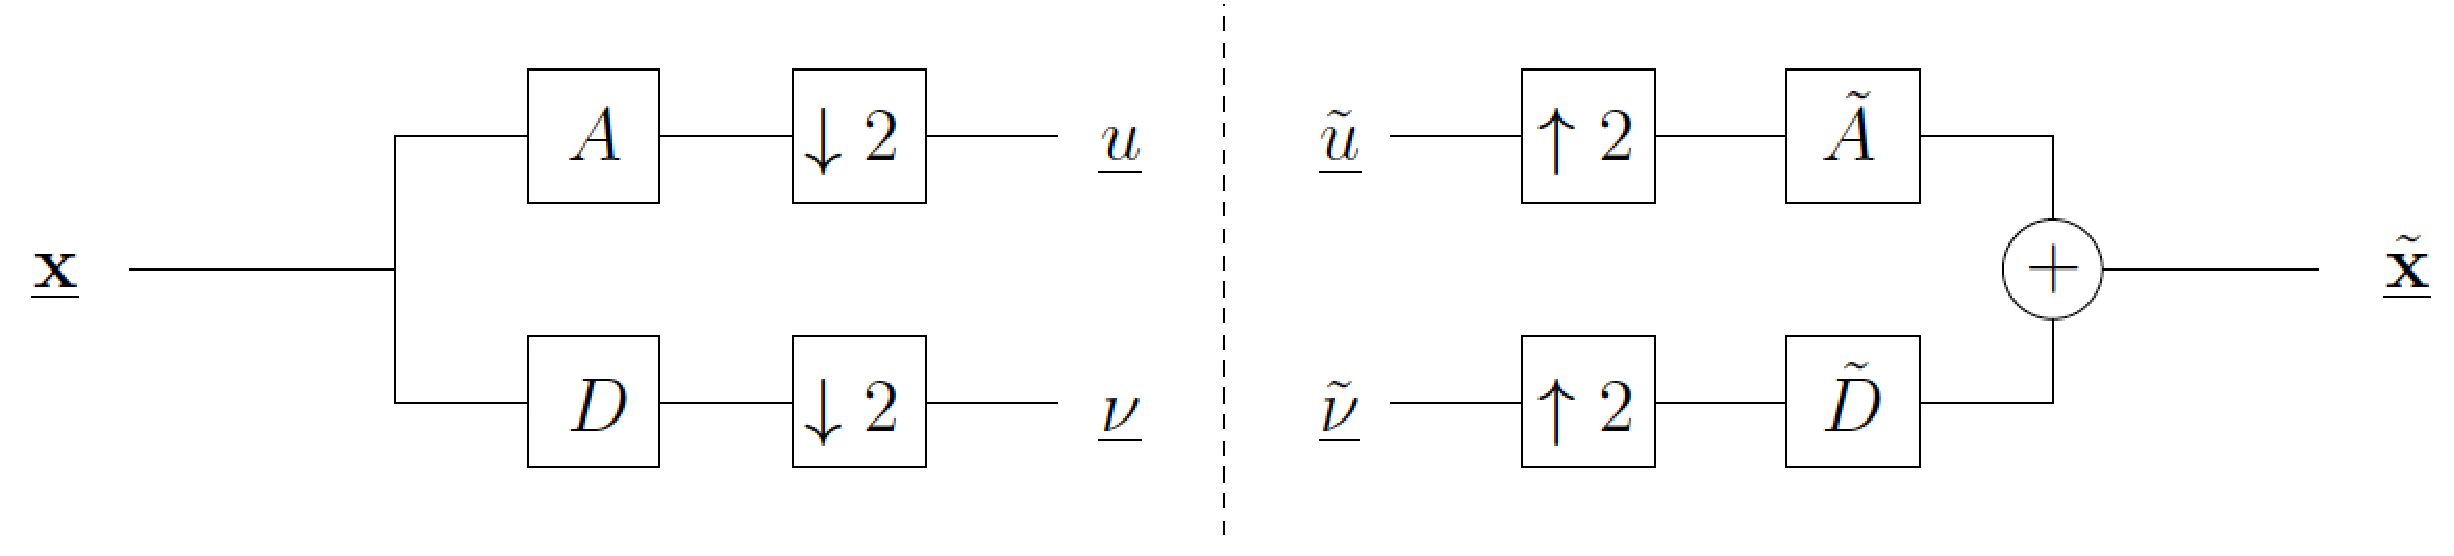
\includegraphics[width=0.5\textwidth]{content/FilterBank.pdf} 
\end{flushright}
 
\vspace{-0.5cm}

Filterbank (durch $-(-1)^k$ werden alle geraden Koeffizienten gelöscht ($=0$) ):
\[  
	\underbrace{\tilde{A}(z) A(z)}_{M(z)} + \underbrace{\tilde{D}(z)D(z)}_{-(-1)^k M(-z)} = M(z)-(-1)^kM(-z) = 2
	\qquad \qquad
	\tilde{A}(z)A(-z) + \tilde{D}(z)D(-z) = 0
\]

(Übung 9 (FS2013)-2a,b): Aus diesen Gleichungen folgt das Gleichungssystem:
\begin{align*}
  \text{Gleichung links, Koeffizient } z^0: \qquad & \tilde a_0 a_0 + \tilde a_1 a_{-1} + \tilde d_0 d_0 + \tilde d_1 d_{-1} &= 2 \\
  \text{Gleichung links, Koeffizient } z^1: \qquad & \tilde a_1 a_0 + \tilde d_1 d_0 &= 0 \\
  \text{Gleichung links, Koeffizient } z^{-1}: \qquad & \tilde a_0 a_{-1} + \tilde d_0 d_{-1} &= 0 \\
  \text{Gleichung rechts, Koeffizient } z^{0}: \qquad & \tilde a_0 a_0 - \tilde a_1 a_{-1} + \tilde d_0 d_0 - \tilde d_1 a_{-1} &= 0 \\
\end{align*}
und daraus die Koeffizienten:
\[
  \begin{pmatrix}
    \tilde a_0 & \tilde a_1\\
    \tilde d_0 & \tilde d_1
  \end{pmatrix}
  = \frac{1}{a_0 d_{-1} - a_{-1} d_0} \begin{pmatrix}
    d_{-1} & -d_0 \\
    -a_{-1} & a_0
  \end{pmatrix}
\]

Perfekte Rekonstruktion mit:
\[
\tilde{X}(z) = \frac12 \left( \big(A(z) X(z) + A(-z)X(-z)\big) \tilde{A}(z) + \big(D(z)X(z) + D(-z)X(-z)\big) \tilde{D}(z) \right)
\]
und im Falle von Haar: 
$A(z) = \frac{1+z}{\sqrt{2}} \quad 
D(z) = \frac{1-z}{\sqrt{2}} \quad 
\tilde{A}(z) = \frac{1+z^{-1}}{\sqrt{2}} \quad 
\tilde{D}(z) = \frac{1-z^{-1}}{\sqrt{2}}$
\\
\subsubsection{Zusammenhang zwischen H, A, D \baeni{76}}
\begin{tabularx}{\textwidth}{X | p{9cm}}
Die Filterkoeffizienten $h_k$ werden so in die Filterbank gerechnet:\newline
$A := H', \, \tilde A := H,\, D := G, \; \tilde D := G$
mit den Koeffizienten: $h'_k = h_{-k}$, $g_k = (-1)^k h_{l-k}$
& Schema: \newline
  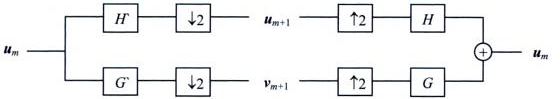
\includegraphics[width=9cm]{./content/MsaFilterbank.png}\\
\end{tabularx}

\subsubsection{Orthogonale Filterkoeffizienten \baeni{52, 75}}
Zusammenhang der Filter (shift: $(-z)^k$, inverse Reihenfolge durch $z^{-1}$, alternierendes Vorzeichen$(\pm)$ durch einsetzen von $-z$):
%TODO wo ist z^0 und wo z^n (Skript seite 27 + application db2 vergleichen???)
\[  
	\tilde{A}(z) = A(z^{-1})
	\qquad \qquad
	D(z) = \tilde{D}(z^{-1}) = (-z)^l\tilde{A}(-z) \qquad l\text{: ungerade, frei wählbar}
\]
\[  
	A = [h_0,...,h_n] \qquad
	\tilde{A} = [h_n,...,h_0]
	\qquad \qquad
	D = [h_n,-h_{n-1}, h_{n-2},...,h_1,-h_0] \qquad
	\tilde{D} = [-h_0,h_1, -h_2,...,-h_{n-1},h_n]
\]

Mit einer orthogonalen Filterbank hat man Quadrature Mirror Filter Eigenschaften:\\
 $|\hat{h}(\xi)|^2 + |\hat{g}(\xi)|^2 = |\hat{\tilde{h}}(\xi)|^2 + |\hat{\tilde{g}}(\xi)|^2 = 2 \qquad \Leftrightarrow \qquad
 |\hat{a}(\xi)|^2 + |\hat{d}(\xi)|^2 = |\hat{\tilde{a}}(\xi)|^2 + |\hat{\tilde{d}}(\xi)|^2 = 2$

\subsubsection{Biorthogonale Filterkoeffizienten}

Zusammenhang der Filter (shift: $(-z)^k$ bzw. $-z^{-k}$, alternierendes Vorzeichen$(\pm)$ durch einsetzen von $-z$):
%TODO wo ist z^0 und wo z^n (Skript seite 27 + application db2 vergleichen???)
\[ 
	D(z) = (-z)^{-l}\tilde{A}(-z^{-1}) \qquad \qquad \tilde{D}(z) = (-z)^{l}A(-z^{-1})  \qquad l\text{: ungerade, frei wählbar}
\]

